\section{Componente per la struttura Phi}
\label{secphi}
L'ottenimento dell'array \textit{matching statistics} permette di sapere solo
l'indice di una della righe del pannello per le quali si ha un match con
l'aplotipo query. Analogamente a quanto discusso in \textit{PHONI} \cite{phoni},
anche per la \textit{RLPBWT} si è pensato a due funzioni, $\boldsymbol\varphi$ e
$\boldsymbol\varphi\mathbf{^{-1}}$, per il riconoscimento di tutte le
righe del pannello per cui si ha il match. La struttura che permette il calcolo
di tali funzioni è la componente denotata \texttt{PHI}.\\
\dc{Qui non ho PLCP quindi calcolo ogni volta}
L'intuizione alla base del ragionamento è molto semplice. Nell'ordinamento alla
colonna $k$-esima, dato da $a_k$, tutte le righe per le quali si ha un match
sono poste consecutivamente, questo a causa del fatto che l'ordinamento è
lessicografico.
\begin{definizione}
  Dati:
  \begin{itemize}
    \item un pannello $X$, di dimensioni $N\times M$
    \item una colonna $k$, il \textit{prefix array} $a_k$ e la sua permutazione
    inversa $\alpha_k$
  \end{itemize}
  Si definiscono formalmente:
  \[\varphi_k(p)=
    \begin{cases}
      null&\mbox{se }\alpha_k[p]=0\\
      a_k[\alpha_k[p]-1]&\mbox{altrimenti}
    \end{cases},\forall p\in\{0,M-1\}
  \]
  \[\varphi^{-1}_k(p)=
    \begin{cases}
      null&\mbox{se }\alpha_k[p]=M-1\\
      a_k[\alpha_k[p]+1]&\mbox{altrimenti}
    \end{cases},\forall p\in\{0,M-1\}
  \]
  In altri termini, avendo $a_k[j]=p$ si ha che:
  \[\varphi_k(p)=
    \begin{cases}
      null&\mbox{se }j=0\\
      a_k[j-1]&\mbox{altrimenti}
    \end{cases},\forall p\in\{0,M-1\}
  \]
  \[\varphi^{-1}_k(p)=
    \begin{cases}
      null&\mbox{se }j=M-1\\
      a_k[j+1]&\mbox{altrimenti}
    \end{cases},\forall p\in\{0,M-1\}
  \]
\end{definizione}
\textbf{VERIFICARE DEFINIZIONE IN QUANTO ``NUOVA''}
\begin{esempio}
  Per praticità si riporta un breve esempio.\\
  Si ipotizzi di avere, come per l'esempio \ref{es:pbwt1}:
  \[a_6=[14,15,0,9,10,16,8,11,12,13,18,19,1,2,3,17,4,5,6,7]\]
  \[\alpha_6=[2,12,13,14,16,17,18,19,6,3,4,7,8,9,0,1,5,15,10,11]\]
  Si fissa quindi $p=3$ e si ottengono:
  \[\varphi(3)=a_6[\alpha_6[3]-1]=a_6[14-1]=a_6[13]=2\]
  \[\varphi^{-1}(3)=a_6[\alpha_6[3]+1]=a_6[14+1]=a_6[15]=17\]
\end{esempio}
Avendo quindi $MS[i].row=p$ e $MS[i].len=l$ basta iterare le righe a partire a
$p$ in $a_i$, che denotiamo con l'indice $q$, fino a che si ha si ha 
$LCE_k(x_p, x_q)\geq l$. Ovviamente bisogna iterare in entrambe le
direzioni. Tutte le righe $x_q$ che soddisfano un match di lunghezza $l$ con
l'aplotipo query. L'algoritmo \ref{algo:phiext} rappresenta esattamente quanto
detto, avendo che con la funzione $lce\_bounded$ si limita il calcolo della
\textit{LCE} alla lunghezza $l$. La complessità temporale di questo algoritmo
varia a seconda della componente \texttt{RA} (e della conseguente presenza della
componente \texttt{LCE}). Inoltre è difficile poter dare una stima asintotica in
quanto varia sul numero di righe che presentano un certo \textit{SMEM}, che
denominiamo qui $\nu$, e dalla lunghezza dello stesso, indicata con
$\lambda$. Quindi, si ha che, qualora si avesse la componente \texttt{RA-BV}, si
avrebbe un tempo proporzionale a:
\begin{equation}
  \label{eq:phiaccbv}
  \mathcal{O}(\nu\lambda)
\end{equation}
Mentre con l'uso della componente \texttt{LCE}, avendo il pannello in memoria
con la componente \texttt{RA-SLP}, si avrebbe una complessità in tempo, con $s$
lunghezza della stringa unica prodotta dall'\textit{SLP}, pari a:
\begin{equation}
  \label{eq:phiaccbv2}
  \mathcal{O}(\nu\lambda\log s)
\end{equation}
\\
\begin{algorithm}
  \begin{algorithmic}[1]
    \Function{extend\_matches}{$k, row, len$}
    \State $haplos\gets []$
    \State $check_{down}\gets \top,\,\,check_{up}\gets \top$
    \While {$check_{down}$}
    \State $down_{row}\gets \varphi^{-1}(row, k)$
    \If{$lce\_bounded(k, row, down_{row}, len)$}
    \State $push(haplos, down_{row})$
    \State $row \gets down_{row}$
    \Else
    \State $check_{down}\gets \bot$
    \EndIf
    \EndWhile
    \While {$up_{down}$}
    \State $up_{row}\gets \varphi(row, k)$
    \If{$lce\_bounded(k, row, up_{row}, len)$}
    \State $push(haplos, up_{row})$
    \State $row \gets up_{row}$
    \Else
    \State $check_{up}\gets \bot$
    \EndIf
    \EndWhile
    \State \textbf{return} $haplos$
    \EndFunction
  \end{algorithmic}
  \caption{Algoritmo per estendere uno SMEM in colonna $k$ usando $\varphi$,
  $\varphi^{-1}$.}
  \label{algo:phiext}
\end{algorithm}
Questa è la definizione formale delle due funzioni ma, all'atto pratico, in
memoria si hanno solo i \textit{prefix array sample}, ad inizio e fine di ogni
run, e nessuna informazione in merito alla \textit{permutazione inversa} del
\textit{prefix array}. Si è quindi pensato ad una struttura dati, basata
anch'essa su \textit{bitvector sparsi}, che permettesse il calcolo delle due
funzioni. 
\subsection{Costruzione della struttura di supporto}
L'idea di base per la costruzione della struttura a supporto delle
\textbf{funzioni} $\boldsymbol\varphi$ e $\boldsymbol\varphi\mathbf{^{-1}}$ si
basa sul fatto che, data una colonna $k$ e dati due valori consecutivi $p$ e $q$
in $a_k$ (avendo $a_k[i]=p$ e $a_k[i+1]=q$), essi rimarranno consecutivi anche
in $a_{k+o}$, \textit{prefix array} dell'arbitraria colonna $k+o$, fino a che
che $x_{p}[k+o]\neq x_{q}[k+o]$, ovvero fino a che, in colonna $k+o$, tali righe
non corrisponderanno a due simboli diversi. Cruciale è che, in quella colonna,
$p$ sarà memorizzato come \textit{prefix array sample} della fine della run $r$
mentre $q$ come \textit{prefix array sample} dell'inizio della run $r+1$. Grazie
a questa informazione si può costruire una struttura che, data una colonna
arbitraria e un arbitrario valore di \textit{prefix array}, permetta di
computare $\varphi$ e $\varphi^{-1}$.\\
Tale struttura dati è composta da:
\begin{itemize}
  \item un vettore di \textit{sparse bitvector} per $\varphi$, che denotiamo con
  $\varPhi$, tale che $\varPhi[i][j]=1$ sse la riga $i$ indicizza una testa di
  run alla colonna $j$ nella \textit{matrice PBWT}. Si ha quindi che $\varPhi$
  ha dimensione $M\times N$
  \item un vettore di \textit{sparse bitvector} per $\varphi^{-1}$, che
  denotiamo con $\varPhi^{-1}$, tale che $\varPhi[i][j]=1$ sse la riga $i$
  indicizza una coda di run alla colonna $j$ nella \textit{matrice PBWT}. Si ha
  quindi che $\varPhi^{-1}$ ha dimensione $M\times N$
  \item un vettore di interi a supporto, denotato $\varPhi_{supp}$, del vettore
  di \textit{sparse bitvector} 
  per $\varphi$ che memorizza, per ogni 1 di tale vettore, il
  \textit{prefix array sample} della coda della run precedente o l'altezza
  del pannello, $M$, qualora non si abbia alcuna run precedente
  \item un vettore di interi a supporto, denotato $\varPhi^{-1}_{supp}$, del
  vettore di \textit{sparse bitvector} 
  per $\varphi^{-1}$ che memorizza, per ogni 1 di tale vettore,
  il \textit{prefix array sample} della testa della run successiva o l'altezza
  del pannello, $M$, qualora non si abbia alcuna run successiva. 
\end{itemize}
Si ha quindi che la lunghezza della riga $i$-esima di $\varPhi_{supp}$ è
uguale al numero di uni presenti nella riga $i$-esima di $\varPhi$. Analogamente
si ha per $\varPhi^{-1}_{supp}$. In entrambi i casi, inoltre, si hanno $M$
righe.\\ 
Al fine della costruzione bisogna, inoltre, sfruttare $a_{N-1}$ per poter
identificare quelle coppie di valori consecutivi non presenti nei vari
\textit{prefix array samples}, in modo che sia possibile effettuare le query per
qualsiasi valore di \textit{prefix array} in input.\\
L'algoritmo \ref{algo:phicos} riporta quindi la costruzione della struttura,
iterando in primis i vari \textit{prefix array samples} e completando i
risultati con $a_{N-1}$. Tale algoritmo ha complessità in tempo, nel caso
peggiore, pari a:
\begin{equation}
  \label{eq:phicos}
  \mathcal{O}(NM)
\end{equation}
Che si ha qualora ogni colonna della \textit{matrice PBWT} abbia un numero di
run pari all'altezza stessa della colonna. Indicando con $\rho$ il numero medio
complessivo di run, si può dire che la complessità nel caso medio è:
\begin{equation}
  \label{eq:phicos2}
  \mathcal{O}(N\rho)
\end{equation}
\textbf{CAPIRE SE COMMENTARE ULTERIORMENTE LA COSTRUZIONE}\\
\begin{algorithm}
  \footnotesize
  \begin{algorithmic}[1]
    \Function{Build\_phi}{$cols, panel, prefix$}
    \Comment  $prefix$ is the last prefix array
    \State $\varPhi\gets [[0..0]..[0..0]],\,\,\varPhi^{-1}\gets
    [[0..0]..[0..0]]$ 
    \Comment sparse bit vector panels for $\varphi$ and $\varphi^{-1}$
    \State $\varPhi_{supp} = [],\,\,\varPhi_{supp}^{-1} = []$
    \Comment vectors for $\varphi$ and $\varphi^{-1}$ row values
    \For {\textit{every} $k\in [0,|cols|)$}
    \For {\textit{every} $i\in [0,|samples_{beg}|)$}
    \State $\varPhi[sample_{beg}^{k}[i]][k]\gets 1$
    \If{$i=0$}
    \State $push(\varPhi_{supp}[sample_{beg}^{k}[i]], panel_{height})$
    \Else
    \State $push(\varPhi_{supp}[sample_{beg}^{k}[i]],sample_{end}^{k}[i-1])$
    \EndIf

    \State $\varPhi^{-1}[sample_{end}^{k}[i]][k]\gets 1$
    \If{$i=|sample_{beg}^k|-1$}
    \State $push(\varPhi_{supp}^{-1}[sample_{end}^{k}[i]], panel_{height})$
    \Else
    \State $push(\varPhi_{supp}^{-1}[sample_{end}^{k}[i]],sample_{beg}^{k}[i+1])$
    \EndIf
    \EndFor
    \EndFor
    \For {\textit{every} $k\in [0,|prefix|)$}
    \If{$\varPhi[k][|\varPhi[k]|-1] = 0$}
    \State $\varPhi[k][|\varPhi[k]|-1]\gets 1$
    \If{$k=0$}
    \State $push(\varPhi_{supp}[prefix[k]], panel_{height})$
    \Else
    \State $push(\varPhi_{supp}[prefix[k]] ,prefix^k[i-1])$
    \EndIf
    \EndIf
    \If{$\varPhi^{-1}[k][|\varPhi[k]|-1] = 0$}
    \State $\varPhi^{-1}[k][|\varPhi[k]|-1]\gets 1$
    \If{$k=|prefix|-1$}
    \State $push(\varPhi^{-1}_{supp}[prefix[k]], panel_{height})$
    \Else
    \State $push(\varPhi^{-1}_{supp}[prefix[k]],prefix^k[i+1])$
    \EndIf
    \EndIf
    \EndFor
    \State \textit{costruzione della struttura rank per ogni bitvector sparso}
    $\varPhi$ e $\varPhi^{-1}$
    \EndFunction
  \end{algorithmic}
  \caption{Algoritmo per la costruzione della componente \texttt{PHI}.}
  \label{algo:phicos}
\end{algorithm}
Dal punto di vista delle query, data una colonna $k$ e un valore di
\textit{prefix array} $p$, si procede quindi nel seguente modo:
\begin{itemize}
  \item per la funzione $\varphi$ si effettua la $rank^\varphi(k)$ sulla riga
  $p$ di $\varPhi$, avendo che:
  \[\varphi_k(p)=
    \begin{cases}
      null&\mbox{se }\varPhi_{supp}^p[rank^\varphi_p(k)]=M\\
      \varPhi_{supp}^p[rank^\varphi_p(k)]&\mbox{altrimenti }
    \end{cases}
  \]
  \item per la funzione $\varphi^{-1}$ si effettua la $rank^{\varphi^{-1}}(k)$
  sulla riga $p$ di $\varPhi^{-1}$, avendo che:
  \[\varphi_k^{-1}(p)=
    \begin{cases}
      null&\mbox{se }\varPhi^{-1\,\,p}_{supp}[rank^{\varphi^{-1}}_p(k)]=M\\
      \varPhi^{-1\,\,p}_{supp}[rank^{\varphi^{-1}}_p(k)]&\mbox{altrimenti }
    \end{cases}
  \]
\end{itemize}
\begin{esempio}
  Si ha la seguente situazione nella \textit{matrice PBWT}:
  \begin{figure}[H]
    \centering
    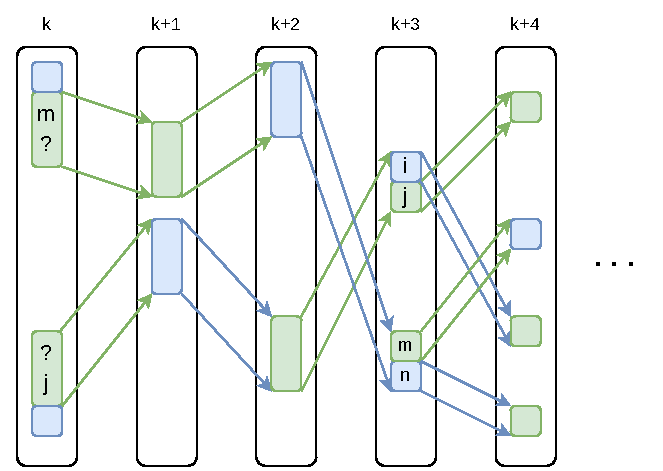
\includegraphics[scale = 0.8]{img/phi.pdf}   
  \end{figure}
  Dove si noti che, a parità di colore, si ha lo stesso simbolo tra due indici
  consecutivi. \\
  In colonna $k$, che per praticità assumiamo essere $k=0$, si vorrebbe avere
  informazione in merito a $\varphi_k(j)$ e $\varphi^{-1}_k(m)$. \\
  Si nota che, per definizione della struttura dati, si ha che (limitandoci alle
  colonne della figura):
  \[\varPhi_j=[0,0,0,1,0, \ldots]\]
  \[\varPhi^{-1}_m=[0,0,0,1,0,\ldots]\]
  In quanto, in entrambi i casi, rispettivamente per la riga $j$ e la riga $m$,
  in colonna $k+3$, si che $j$ è il \textit{prefix array} di una testa di run
  mentre $m$ di una coda di run. In colonna $k+3$ si conoscono anche,
  rispettivamente, $i$, \textit{prefix array} della coda della run precedente a
  quella di $j$, e $n$, \textit{prefix array} della testa della run successiva
  quella di $m$. Si ottengono quindi:
  \[\varPhi_{supp}=[i,\ldots]\]
  \[\varPhi^{-1}_{supp}=[n,\ldots]\]
  Si vogliono quindi calcolare $\varphi_0(j)$ e  $\varphi^{-1}_0(m)$. Si ha:
  \[\varPhi_{supp}^j[rank^\varphi_j(0)]=\varPhi_{supp}^j[0]=i\]
  \[\varPhi^{-1\,\,m}_{supp}[rank^{\varphi^{-1}}_m(0)]=\varPhi^{-1\,\,m}_{supp}[0]=n\]
  Si noti che uguali risultati si avrebbero per $k+1$, $k+2$ e $k+3$.
\end{esempio}
\dc{SISTEMARE UN PO' TUTTO}